% Interpretability example for COVER: alignment, per-word support/conflict and the logical
% aggregation. Values are ILLUSTRATIVE (computed by hand to be consistent with the equations of
% Sec. 3.2); replace them with node-level scores exported from a trained model.
% Included with \includestandalone (sections/results.tex); also compiles alone.
\documentclass[tikz,border=3pt]{standalone}
\usepackage[T1]{fontenc}
\usepackage{newtxtext,newtxmath}
\usetikzlibrary{positioning,arrows.meta,calc}

\definecolor{neural}{HTML}{2F6DB5}
\definecolor{neuralbg}{HTML}{E8F0FA}
\definecolor{logic}{HTML}{2E8B57}
\definecolor{logicbg}{HTML}{E6F4EC}
\definecolor{symb}{HTML}{D9822B}
\definecolor{relneg}{HTML}{C0392B}

\tikzset{
  tok/.style={draw=neural!80, fill=white, rounded corners=1.5pt, inner sep=1.6pt, font=\scriptsize,
              minimum height=4mm, anchor=base},
  htok/.style={tok, fill=neural!12},
  stok/.style={tok, draw=black!25, text=black!45},
  aedge/.style={line width=#1, draw=logic},
  cedge/.style={line width=#1, draw=relneg},
  ledge/.style={line width=#1, draw=neural, densely dashed},
  rlab/.style={font=\tiny, fill=white, inner sep=0.6pt},
  bar/.style={draw=none},
}

% \bars{x}{support}{conflict}{omega}: support (green) and conflict (red) bars under a hypothesis word
\newcommand{\bars}[4]{%
  \fill[logic]  (#1-0.17,0.05) rectangle ++(0.15,{0.8*#2});
  \fill[relneg] (#1+0.02,0.05) rectangle ++(0.15,{0.8*#3});
  \node[font=\tiny, anchor=north] at (#1-0.095,0.03) {$s$};
  \node[font=\tiny, anchor=north] at (#1+0.095,0.03) {$c$};
  \node[font=\tiny, anchor=north] at (#1,-0.22) {$#2\,/\,#3$};
  \node[font=\tiny, anchor=north, text=black!60] at (#1,-0.47) {$\omega{=}#4$};
}

% Paper macros, for standalone compilation (the paper's definitions take precedence).
\providecommand{\Pcov}{P_{\mathrm{cov}}}
\providecommand{\Pnc}{P_{\neg\mathrm{conf}}}
\providecommand{\E}{\textsc{e}}
\providecommand{\N}{\textsc{n}}
\providecommand{\C}{\textsc{c}}

\begin{document}
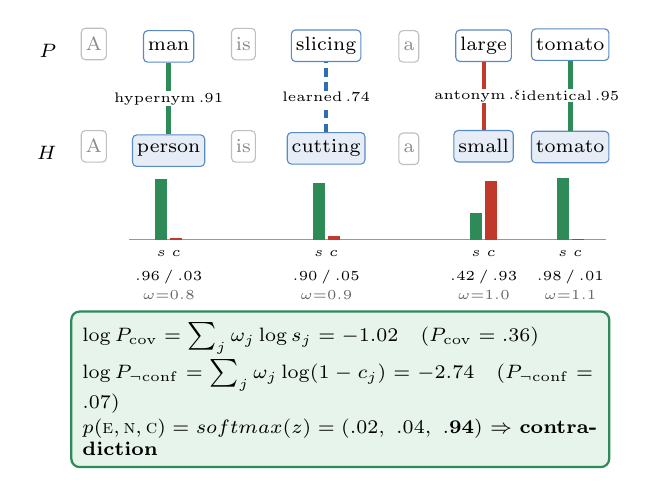
\begin{tikzpicture}

% ---------------------------------------------------------------- premise / hypothesis
\node[font=\scriptsize\itshape, anchor=east] at (-0.35,2.45) {$P$};
\node[font=\scriptsize\itshape, anchor=east] at (-0.35,1.15) {$H$};

\foreach \x/\w/\s [count=\i] in {0/A/stok, 0.95/man/tok, 1.9/is/stok, 2.95/slicing/tok, 4.0/a/stok,
                                 4.95/large/tok, 6.05/tomato/tok}
  \node[\s] (p\i) at (\x,2.45) {\w};
\foreach \x/\w/\s [count=\i] in {0/A/stok, 0.95/person/htok, 1.9/is/stok, 2.95/cutting/htok, 4.0/a/stok,
                                 4.95/small/htok, 6.05/tomato/htok}
  \node[\s] (h\i) at (\x,1.15) {\w};

% ---------------------------------------------------------------- alignment (width ~ attention)
\draw[aedge=1.6pt] (h2.north) -- node[rlab, pos=0.5] {hypernym\,.91} (p2.south);
\draw[ledge=1.2pt] (h4.north) -- node[rlab, pos=0.5] {learned\,.74} (p4.south);
\draw[cedge=1.5pt] (h6.north) -- node[rlab, pos=0.5] {antonym\,.88} (p6.south);
\draw[aedge=1.7pt] (h7.north) -- node[rlab, pos=0.5] {identical\,.95} (p7.south);

% ---------------------------------------------------------------- per-word support / conflict
\draw[black!40] (0.45,0.05) -- (6.5,0.05);
\bars{0.95}{.96}{.03}{0.8}
\bars{2.95}{.90}{.05}{0.9}
\bars{4.95}{.42}{.93}{1.0}
\bars{6.05}{.98}{.01}{1.1}

% ---------------------------------------------------------------- aggregation
\node[draw=logic, fill=logicbg, rounded corners=3pt, line width=0.8pt, font=\scriptsize, align=left,
      anchor=north west, text width=6.55cm, inner sep=4pt] (agg) at (-0.3,-0.85) {%
  $\log\Pcov=\sum_j\omega_j\log s_j=-1.02$\quad($\Pcov=.36$)\\[1pt]
  $\log\Pnc=\sum_j\omega_j\log(1-c_j)=-2.74$\quad($\Pnc=.07$)\\[1pt]
  $p(\E,\N,\C)=\operatorname{softmax}(z)=(.02,\ .04,\ \mathbf{.94})$ $\Rightarrow$ \textbf{contradiction}};

\end{tikzpicture}
\end{document}
